\chapter{ディレクトリとパス}

\section*{ファイル・システムの全体像}

 UNIX システムでは、ファイル・システムは、ツリー状の階層化ディレクトリ構造を
している。

これは簡単に言うと次のようになる。
\begin{enumerate}
\item たくさんあるファイルを、種類ごとに「\textbf{ディレクトリ}」と
呼ばれる箱に分けてしまうことで整理する。
\item \textbf{ディレクトリ}の中にも、また\textbf{ディレクトリ}を作ることができ、
更に細かく分類して整理できる。
\item \textbf{ディレクトリ}の構造図を書くと、木が枝をひろげたよう(ツリー状)に見える。
\end{enumerate}

このようなディレクトリ構造は、後に MS-DOS や Windows などにも採り入れられた。
 Windows では、「ディレクトリ」のことを「フォルダ」と呼んでいる。

\bigskip

 UNIX システムには、いろいろなファイルやコマンドがある。
ディレクトリの中を自由に移動できるようになれば、
これらのことを詳しく知ることができるようになる。
また、自分のファイルをディレクトリに分けてしまっておくと、
きれいに整理されて、便利に使うことができるようになる。

この章では、ディレクトリの移動、作成、消去などについて紹介しよう。

\section{UNIX システムのディレクトリ構造}

\subsection{ディレクトリの全体像}

最初に UNIX システムの全体像を紹介してしまう。

次のページの図 \ref{dirstru} は、 UNIX のディレクトリ構造の主な部分を書いた
ものである。
これには、次のようなディレクトリがある。

\begin{itemize}
\setlength{\parindent}{1zw}
\item \textbf{\large ルート・ディレクトリ /}

一番上のディレクトリを「\textbf{ルート・ディレクトリ}」といい、
「\texttt{/}」で表す。
なお、「ルート -- root 」というのは「(木の)根」のことだ。

ルートの下には、「\texttt{home}」、「\texttt{bin}」、「\texttt{etc}」など、
いろいろなディレクトリが、枝をひろげている。
そして、それらのディレクトリの先にも、またディレクトリがあり、
さらに枝がひろがっている。

これらがツリー状に見える。
絵としては、木が上下さかさまに描かれていると思ってくれればいい。

\begin{figure}[H]
\centering{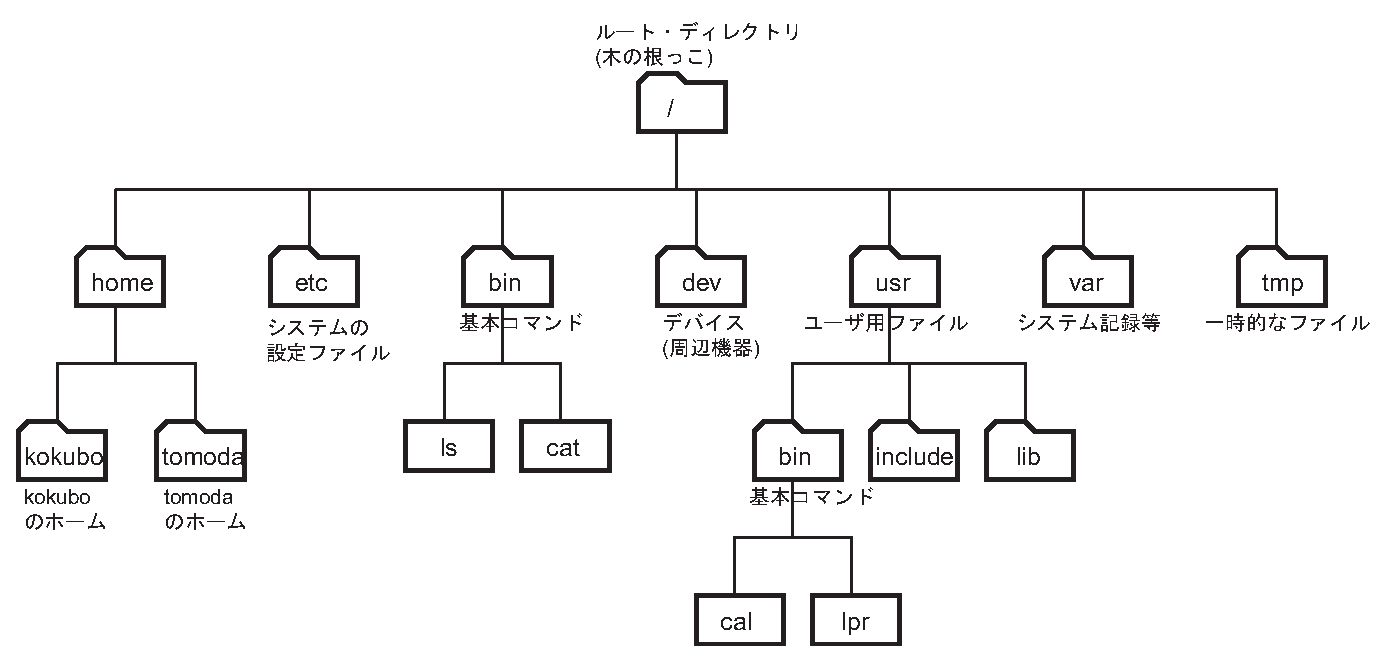
\includegraphics[scale=0.7]{unixtree.eps}}
\caption{UNIX システムのディレクトリ構造}\label{dirstru}
\end{figure}

では、ルート・ディレクトリの下を一つずつ説明していこう。

\item \textbf{\large ホーム・ディレクトリ home}

まず、「\texttt{/}」の下には、「\texttt{home}」というディレクトリがあり、
この中にユーザ ID と同じ名前のついたディレクトリがある。
これらは、 UNIX システムで「\textbf{ホーム・ディレクトリ}」と呼ばれている。

たとえば上の図では、 \texttt{kokubo} さんのホーム・ディレクトリは、
「\texttt{/}」の下の「\texttt{home}」の下の「\texttt{kokubo}」になる。
これを、「\texttt{/home/kokubo}」と表す。
このようにディレクトリの区切りを表すマークは「\texttt{/}」である。

また同様に、 \texttt{tomoda} さんのホーム・ディレクトリは、「\texttt{/}」
の下の「\texttt{home}」の下の「\texttt{tomoda}」で、
これを「\texttt{/home/tomoda}」と表す。

\bigskip

 login した直後、それぞれのユーザは、自分のホーム・ディレクトリにまず入る。
これまでの演習で作ったファイルも、みんな自分のホーム・ディレクトリに
あるはずである。

上の例では、 \texttt{kokubo} さんは login すると、
「\texttt{/home/kokubo}」に入る。
そして、これまでの演習で \texttt{kokubo} さんが作ったファイルは、
そこに置いてあるということだ。

\item \textbf{\large bin}

「\texttt{/}」の下の「\texttt{bin}」、つまり「\texttt{/bin}」には、
 UNIX システムの一番基本的なコマンド
(たとえば \texttt{ls} や \texttt {cat} など)が置いてある。

「\texttt{bin}」というのは「バイナリ -- binary」の略で、
本来は文字ではないデータが入っているファイルのことを意味する
\footnote{マシン語で書かれたコマンドや、画像、音声データなどが、
本来の意味ではバイナリである}。

\item \textbf{\large etc}

「\texttt{etc}」は「エトセトラ -- etc.」である。
 UNIX システムのシステム設定用のファイルが置かれている。

\item \textbf{\large tmp}

「\texttt{tmp}」は「テンポラリ -- temporary」である。
主に、システムが一時的にファイルを作るときに、ここを使う。

\item \textbf{\large usr}

「\texttt{usr}」は「ユーザ -- user」という意味だ。

この中は更に分かれていて、「\texttt{/usr/bin}」にはユーザが使う各種コマンド、
「\texttt{/usr/include}」には C 言語のヘッダ・ファイル、
「\texttt{/usr/lib}」にはユーザ・コマンドが使うライブラリと呼ばれているデータ
などが置かれている。

\item \textbf{\large var}

「\texttt{var}」は「変化する -- variable」という意味だ。
 login をはじめとするシステムの記録、メールなど、
日々変化するデータが置かれている。
\end{itemize}

\newpage

\subsection{B 演習室の実際}

ここまで紹介してきたのは、あくまでも標準のスタイルである。
ディレクトリの構造は、システムの管理者の好みに応じて
変えることもできる。

\bigskip

B 演習室では、ホーム・ディレクトリの様子は、図 \ref{Benshu} のように
変更されている。
なお、ホーム・ディレクトリ以外は標準の構成のままである。

図を見てもらうとわかるが、「\texttt{/}」の下に「\texttt{home}」があるところ
までは一緒である。
違うのは、更にこの中が入学年度別に「\texttt{ei00}」、
「\texttt{ei01}」、「\texttt{ei02}」、「\texttt{ei03}」・・・と
切り分けてあるところだ。

\bigskip

そして、この中にそれぞれのユーザのホーム・ディレクトリがある。

たとえば、 \texttt{ei00000} さんのホーム・ディレクトリは
「\texttt{/home/ei00/ei00000}」だ。
同様に \texttt{ei01001} さんは「\texttt{/home/ei01/ei01001}」となる。

自分のホーム・ディレクトリの中には、これまでの演習で作った
「\texttt{kongetsu}」、「\texttt{renshuu1}」などのファイルが
入っている。

\bigskip

また、後の方で説明するが、ユーザはホーム・ディレクトリの中に
「\texttt{report}」や「\texttt{prog}」などのディレクトリを、
自分で自由に作ってファイルを整理することができる。

\begin{figure}[H]
\centering{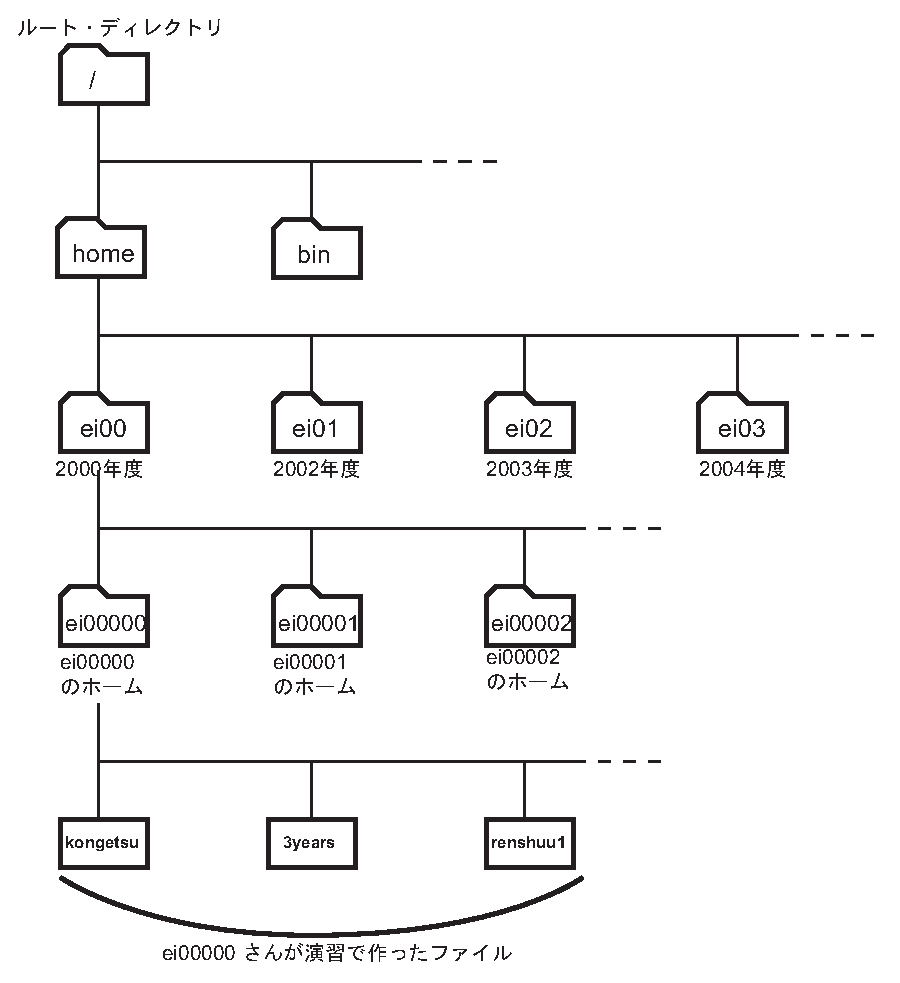
\includegraphics[scale=0.8]{Broom.eps}}
\caption{B 演習室の実際のホーム・ディレクトリの構造}\label{Benshu}
\end{figure}

\section{パス}

 UNIX システムでは、
ファイルやディレクトリの場所を指定するのに、
「\textbf{パス}」を使う。

「パス -- path」というのは、「通り道」や「経路」という意味だ。
パスには、「\textbf{絶対パス}」と「\textbf{相対パス}」がある。

このパスをマスターすることで、好きな場所に移動して UNIX の中を探検したり、
ファイルを好きな場所にコピーしたりすることができる\footnote{セキュリティ上、
いじれないようになっている場所もある。}ようになる。

パスは UNIX システムをマスターする上で、最重要ポイントの一つだ。

\subsection{根っこからの通り道: 絶対パス}

既に、ここまでのところで紹介してしまったが、
「\texttt{/home/kokubo}」のように、 \underline{一番上のルート・}\\
\underline{ディレクトリから、ひとつずつ順番に書いて表す}
方法を、\textbf{「絶対パス」}と呼ぶ。

\begin{figure}[H]
\centering{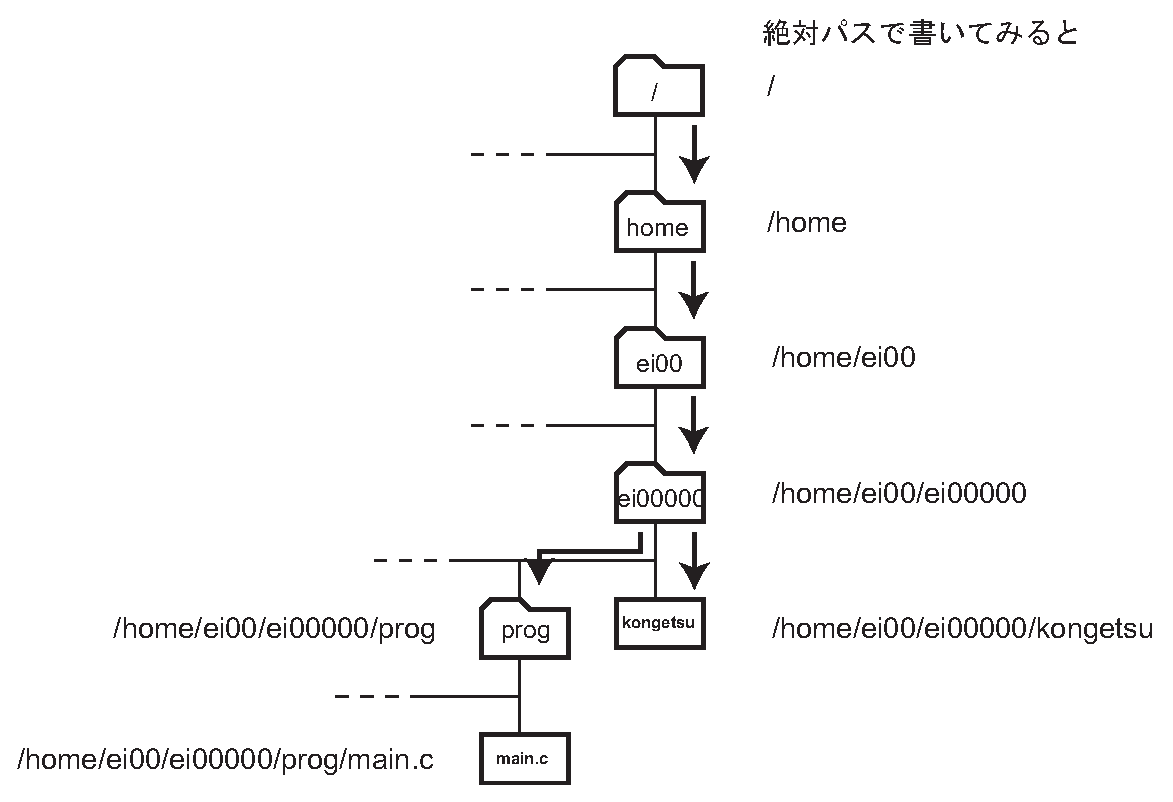
\includegraphics[scale=0.8]{absolutepath.eps}}
\caption{絶対パスでの表し方}\label{absol}
\end{figure}

図 \ref{absol} を使って説明しよう。
まず、一番上にルート・ディレクトリがあり、
これは絶対パスで表すと「\texttt{/}」になる。

「\texttt{/}」の下には「\texttt{home}」があって、
これは絶対パスでは「\texttt{/home}」となる。

その下は学年ごとにディレクトリが用意されていて、「\texttt{ei00}」は
絶対パスでは「\texttt{/home/ei00}」となる。

たとえばその中に、 \texttt{ei00000} さんのホーム・ディレクトリがあって、
これは「\texttt{/home/ei00/ei00000}」だ。

そして、 \texttt{ei00000} さんは、自分のホーム・ディレクトリの中に
「\texttt{kongetsu}」というファイルを作ることができて、
これは「\texttt{/home/ei00/ei00000/kongetsu}」と表される。
同様に「\texttt{renshuu1}」は「\texttt{/home/ei00/ei00000/renshuu1}」
と表される。

このように\underline{一番上の根っこ(ルート・ディレクトリ)から順番に、書いていくのが絶対パス}である。

\bigskip

ここで、注意しておいて欲しいのは、
 \underline{UNIX のパスでは「ファイル」も「ディレクトリ」も全く同じ}\\{
\underline{ように表される}ということだ。
たとえば、図 \ref{filedir} の「\texttt{kongetsu}」はファイルである。
これを絶対パスで表すと「\texttt{/home/ei00/ei00000/kongetsu}」になる。
ところが、「\texttt{kongetsu}」がディレクトリであっても
絶対パスで書けば同様に「\texttt{/home/ei00/ei00000/kongetsu}」になる。

\begin{figure}[H]
\centering{
\includegraphics[scale=0.8]{filedir.eps}}
\caption{ファイルでもディレクトリでもパスは同じ}\label{filedir}
\end{figure}

これは UNIX では、普通のファイル、ディレクトリ、周辺機器(画面、
プリンタ、ネットワーク・カード、その他)などのさまざまなものを、
統一的に「ファイル」として取り扱っているためである。
このようになっていると、プログラムを書いたりするときに、
これらのさまざまなものをだいたい同じような方法で取り扱う
ことができるという利点がある。 

\newpage

\subsection{自分がいるところが中心: 相対パス}

絶対パスを使って、ルート・ディレクトリから順番に書いていけば、
どんなディレクトリでも表せる。
ところが、ディレクトリが下の方になってくると、
どんどん長くなっていき面倒になる。

\bigskip

そこで、 UNIX システムでは、\textbf{「相対パス」}という、
もう一つの方法が用意されている。
相対パスでは、俺が世界の中心という感じで、
「自分が今いるところ」を基準にして指定する。

\bigskip

では、図 \ref{relative0} を見ながら説明しよう。

まず、 \texttt{ei00000} さんは、今自分のホーム・ディレクトリ
である「\texttt{/home/ei00/ei00000}」にいるとしよう。

この中に「\texttt{kongetsu}」というファイルがあるとする。
これは相対パスでは単に「\texttt{kongetsu}」と書く。
絶対パスだと「\texttt{/home/ei00/ei00000/kongetsu}」と
長くなってしまうが、相対パスだと簡単になる。

また、ホーム・ディレクトリの中に「\texttt{prog}」という
ディレクトリがあるとしよう。
これも相対パスでは「\texttt{prog}」となり、とても簡単に書ける。

更に、「\texttt{prog}」の中に、「\texttt{main.c}」という
ファイルがあるとする。
これは相対パスでは「\texttt{prog/main.c}」である。

このように相対パスとは、
\underline{自分が今いるところから、順番にパスを書いていく}方法である。

\bigskip

なお、絶対パスと相対パスの見分け方は簡単で、\underline{最初が「\texttt{/}」で
はじまっていれば絶対パス}である。

\bigskip

\begin{figure}[H]
\centering{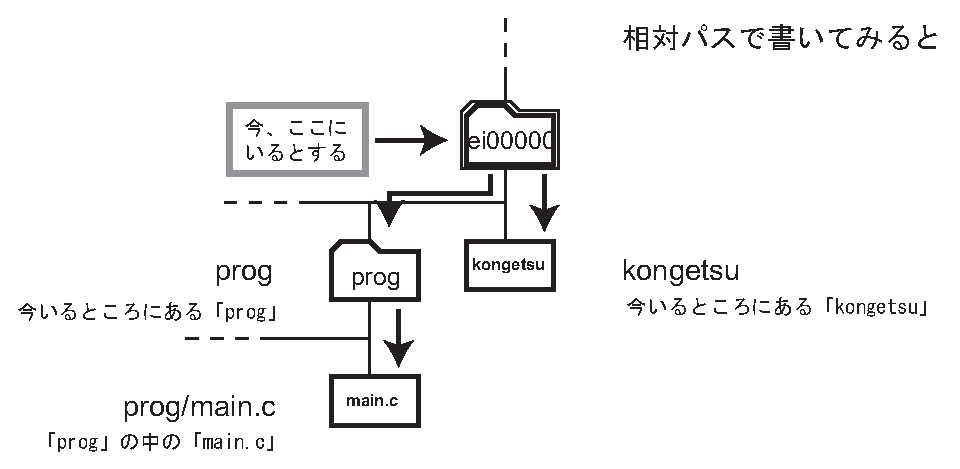
\includegraphics[scale=0.8]{relativepath0.eps}}
\caption{下にあるファイルやディレクトリを相対パスで表す}\label{relative0}
\end{figure}

\newpage

\subsubsection{自分が今いるディレクトリ: 「\texttt{.}」}

\textbf{自分が今いる場所}は、相対パスでは「\texttt{.}」と、
ピリオド 1 つで表わす。

図\ref{relative3} を見てみよう。
今、「\texttt{/home/ei00/ei00000}」にいるとする。
ここは相対パスで表すと「\texttt{.}」となる。

\begin{figure}[H]
\centering{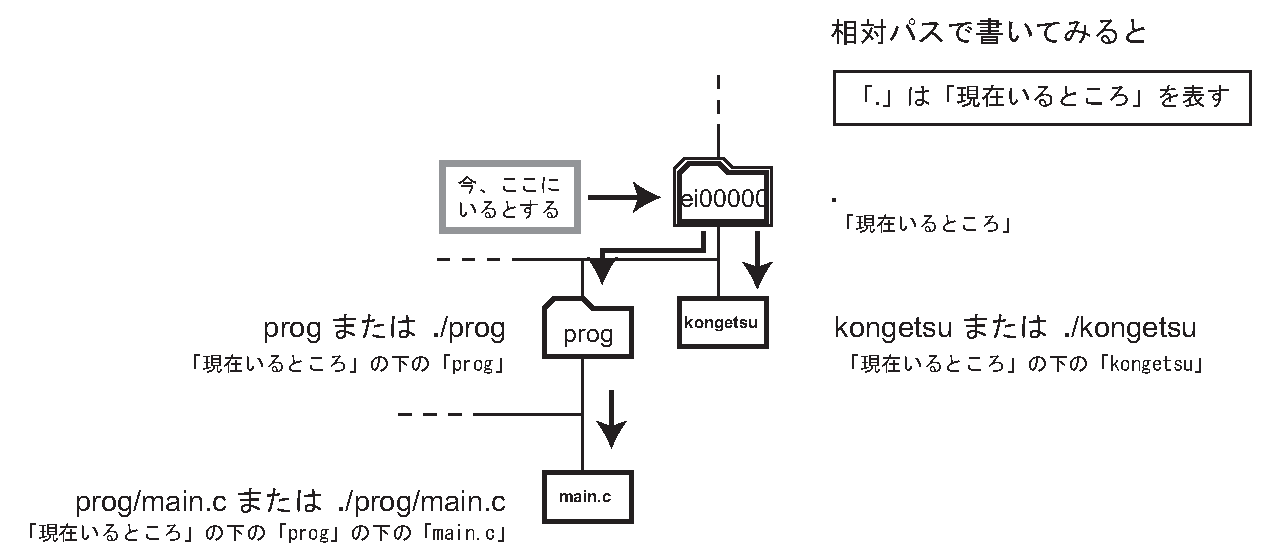
\includegraphics[scale=0.8]{relativepath03.eps}}
\caption{自分のいるディレクトリを相対パスで表す}\label{relative3}
\end{figure}

また、さきほど「\texttt{kongetsu}」は相対パスで
「\texttt{kongetsu}」と書くと紹介した。
これは、「現在いるところ」の下の「\texttt{kongetsu}」と見ることもできて、
「\texttt{./kongetsu}」というふうにも表せる。

同様に「\texttt{prog}」は「\texttt{./prog}」、
「\texttt{prog/main.c}」は「\texttt{./prog/main.c}」とも表せる。

\subsubsection{1つ上のディレクトリ: 「\texttt{..}」}

ここまでは自分よりも下のディレクトリの表し方を紹介してきた。
では、逆に上の方はどうなるのかを紹介しよう。

図 \ref{relative1} を見てみよう。
 UNIX システムでは、 「一つ上」のディレクトリは「\texttt{..}」と表す。
つまり、自分のホームの一つ上の「\texttt{/home/ei00}」は、
「\texttt{..}」と表される。

この\textbf{「ピリオド 2 つで、 1 つ上」}は、とてもよく使うので覚えておこう。

\bigskip

では、 2 つ上はどうか？

1 つ上が「\texttt{..}」で、ディレクトリの区切りが「\texttt{/}」なので、
2 つ上は「\texttt{../..}」となる。
つまり、「\texttt{/home}」は、相対パスでは「\texttt{../..}」となる。
同様にルート・ディレクトリ「\texttt{/}」は、相対パスでは
「\texttt{../../..}」である。

\begin{figure}[H]
\centering{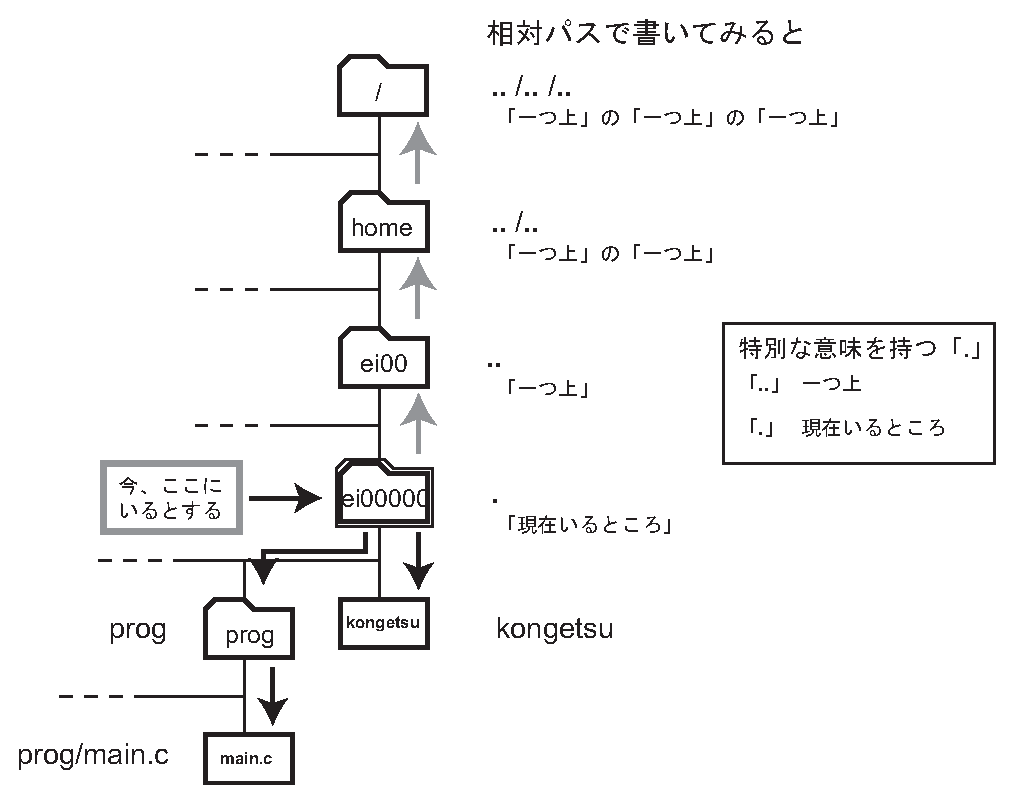
\includegraphics[scale=0.8]{relativepath02.eps}}
\caption{上にあるファイルやディレクトリを相対パスで表す}\label{relative1}
\end{figure}

\newpage

\subsubsection{自分のいる場所によって相対パスは変わる}

ここまでの例は、あくまで「\texttt{/home/ei00/ei00000}」にいる
場合の話である。

相対パスは自分が今いるところを中心に指定するので、
別なディレクトリにいる場合、話が全く変わってくる。

\bigskip

たとえば、図 \ref{relative4}のように
「\texttt{/home/ei00/ei00000/prog}」にいるとしよう。

今度は、自分のホーム・ディレクトリは一つ上にあり、
これは相対パスでは「\texttt{..}」となる。

また、「\texttt{main.c}」は、今いるところのすぐ下にあるので、相対パスでは
「\texttt{main.c}」になる。

\bigskip

このように相対パスは、現在どこのディレクトリに自分がいるかによって
変わってしまう。

\begin{figure}[H]
\centering{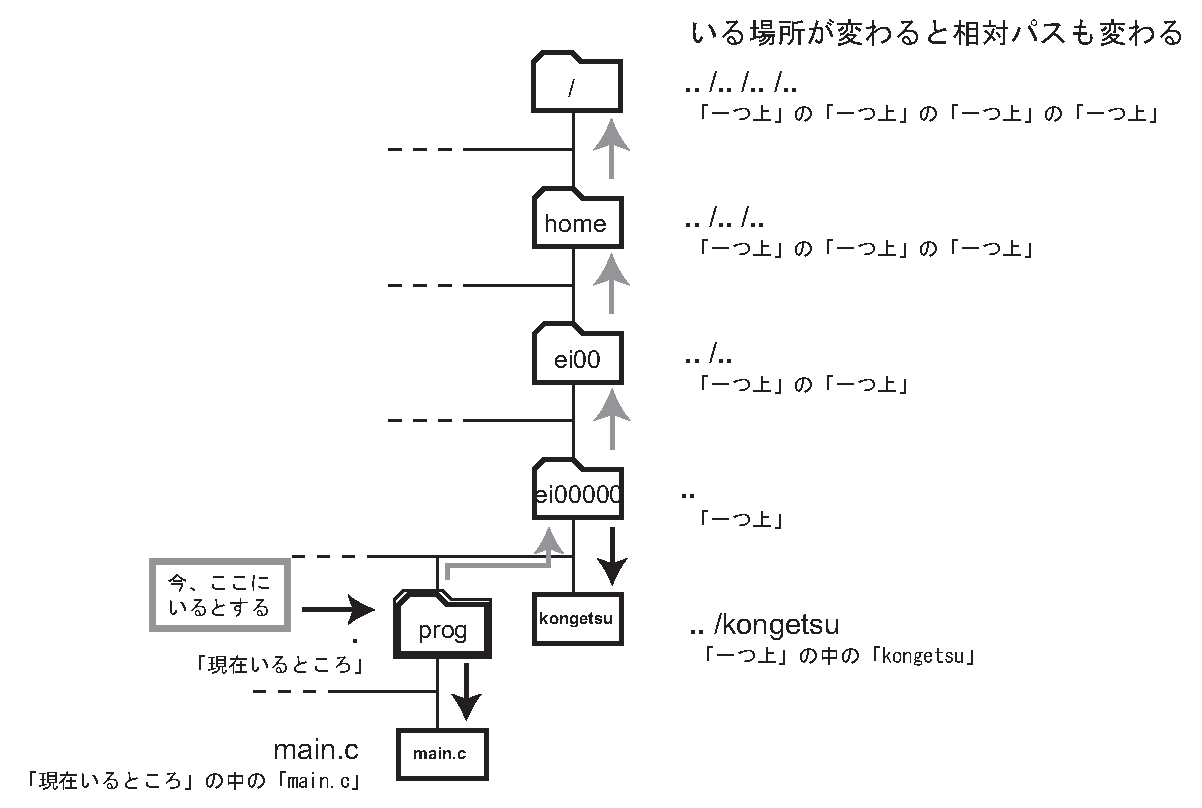
\includegraphics[scale=0.8]{relativepath04.eps}}
\caption{\texttt{prog}の中にいるときの相対パス}\label{relative4}
\end{figure}

\subsection{絶対パスと相対パス、どっちがお特?}

 UNIX システムでは、絶対パスで指定しても、相対パスで指定しても、
効果は全く同じである。

だから、自分で好きな方を使っていい。

ただし、自分が今いるところの近くを指定するには「相対パス」を、
ルート・ディレクトリの近くを指定するには「絶対パス」を使った方が簡単である。

このように使い分けるので、両方を知っておいた方が便利だ。

\newpage
\noindent
\textbf{\large ☆練習☆}

下の図にそれぞれ相対パスを記入しよう。

\begin{figure}[H]
\centering{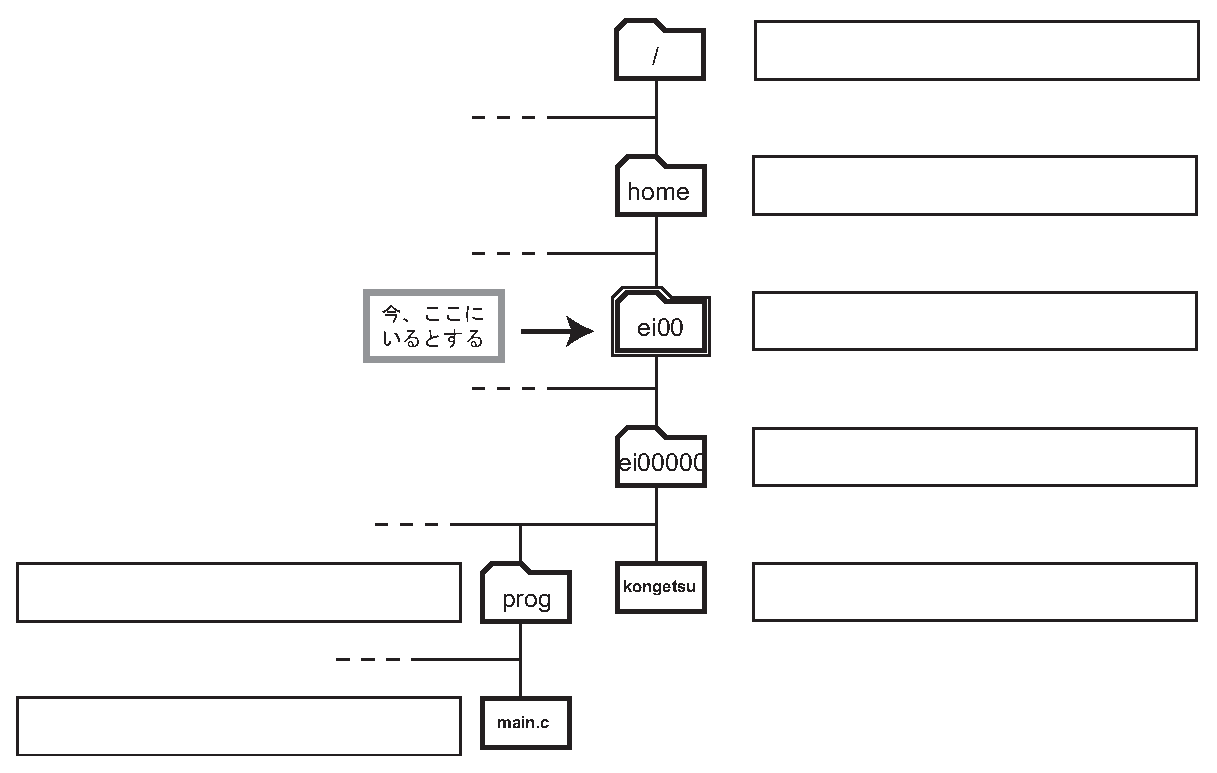
\includegraphics[scale=0.8]{relativepath06.eps}}
\end{figure}

解答はこの章の最終ページにある。

\newpage

\section{ディレクトリ操作コマンド}

では、具体的に、コマンドを使ってディレクトリを移動したり、
ディレクトリを作ったりしてみよう。

\subsection{現在いるディレクトリの表示: \texttt{pwd}}

login した直後にいる場所が、自分のホーム・ディレクトリであると、
前の方で説明した。
では、それがどこか見てみよう。

今いるディレクトリを表示するには、 \texttt{pwd} コマンドを使う。
 \texttt{pwd} は「\textbf{p}rint \textbf{w}orking \textbf{d}irectory」の略で、
「今お仕事をしているディレクトリを表示」という意味だ。

使い方は、単に次のように打てばいい。

\begin{coml}{2cm}
\texttt{pwd}
\end{coml}

さて、図 \ref{nowlogged} のようなディレクトリ構造だとしよう。
\texttt{ei00000} さんは、今 login した直後で、
ホーム・ディレクトリの「\texttt{/home/ei00/ei00000}」にいるとしよう。
このとき、 \texttt{pwd} を実行すると、

\begin{progls}
% \slbfl{pwd}
/home/ei00/ei00000
%
\end{progls}

となり、 今いるのが「\texttt{/home/ei99/ei99000}」だと表示される。

\begin{figure}[H]
\centering{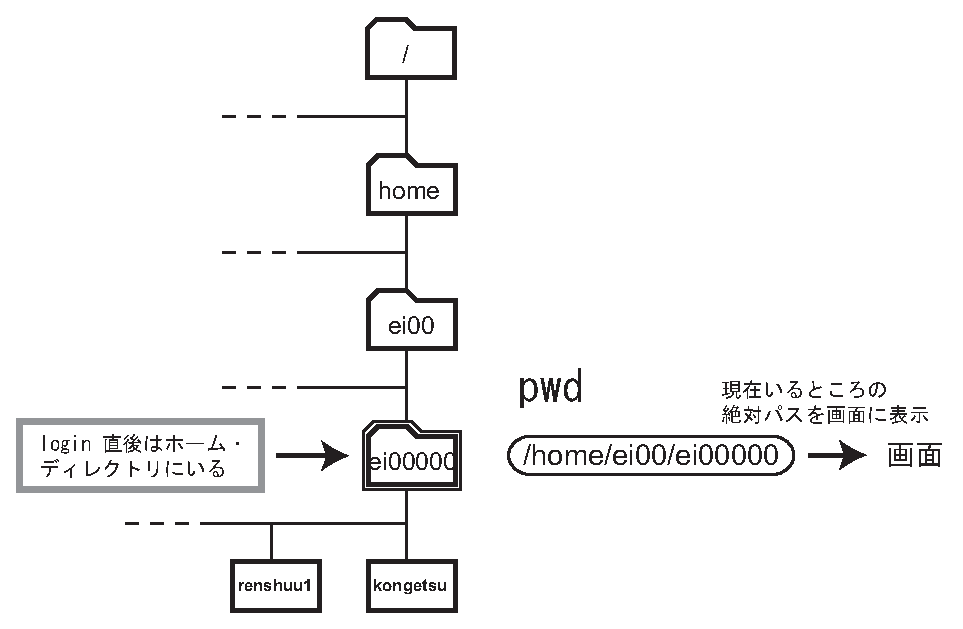
\includegraphics[scale=0.8]{pwd.eps}}
\caption{login 直後の ei00000 さん}\label{nowlogged}
\end{figure}

\newpage

\subsection{ディレクトリを移動: \texttt{cd}}

では、ディレクトリの冒険の旅に出かけよう。
ディレクトリを移動するには、 \texttt{cd} を使う。
これは「\textbf{c}hange \textbf{d}irectory -- チェンジ・ディレクトリ」の略だ。
使い方は以下の通り。
この「パス」というのは、絶対パス、相対パスのどちらでもいい。

\begin{coml}{3.5cm}
\texttt{cd} 「パス」
\end{coml}

\noindent

\subsubsection{ 1 つ上へ移動}

では、 1 つ上のディレクトリに移動してみよう。

現在は「\texttt{/home/ei00/ei00000}」にいる。
よって、 1 つ上のディレクトリは、絶対パスでは「\texttt{/home/ei00}」となり、
相対パスでは「\texttt{..}」となる。
よって 1 つ上に移動するには、「\texttt{cd /home/ei01}」、
または「\texttt{cd ..}」のどちらでもいい。

この場合、明らかに「\texttt{cd ..}」の方が楽なので、こちらを実行する。

\begin{progls}
% \slbfl{cd ..}
%
\end{progls}

これで、ディレクトリを一つ登れた。
 \texttt{pwd} で確認してみよう。

\begin{progls}
% \slbfl{pwd}
/home/ei00
%
\end{progls}

確かに、「\texttt{/home/ei00}」にいることがわかる。

\begin{figure}[H]
\centering{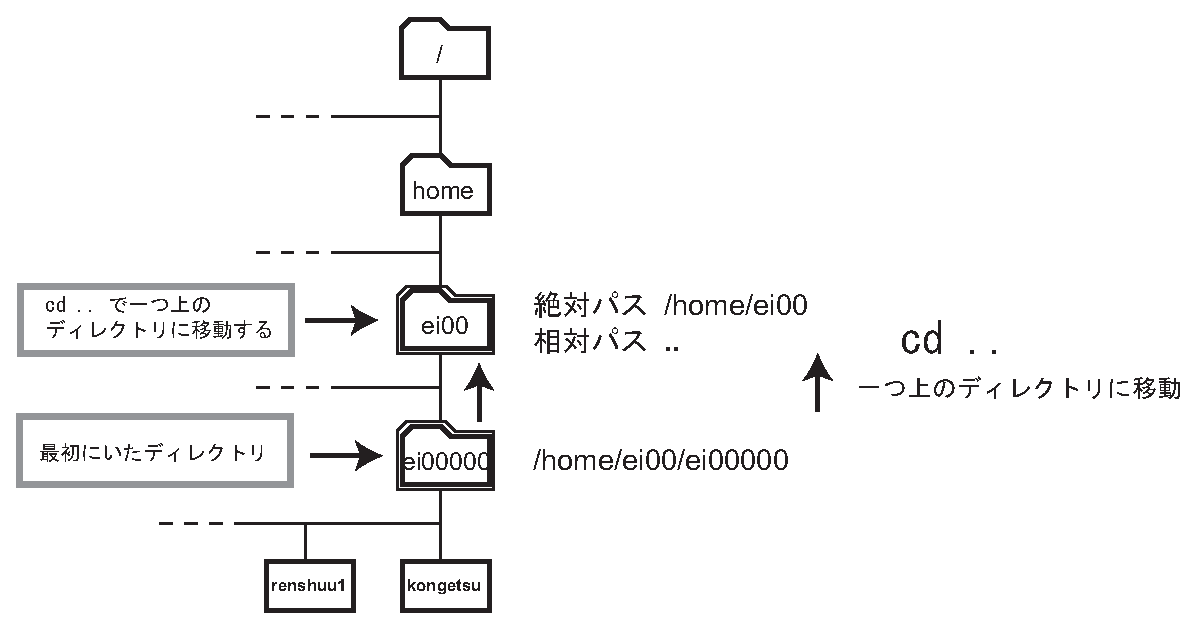
\includegraphics[scale=0.8]{cdup.eps}}
%\caption{「\texttt{cd ..}」で一つ上へ}\label{cdup}
\end{figure}

\bigskip

では、ここにどんなファイルがあるか \texttt{ls} で見てみよう。
すると、同級生のホーム・ディレクトリのリストが見える。

\begin{progls}
% \slbfl{ls}
ei00001 ei00006 ei00011 ei00016 ei00021 ei00026 ei00031 ei00036 ei00041
ei00002 ei00007 ei00012 ei00017 ei00022 ei00027 ei00032 ei00037 ei00042
ei00003 ei00008 ei00013 ei00018 ei00023 ei00028 ei00033 ei00038 ei00043
ei00004 ei00009 ei00014 ei00019 ei00024 ei00029 ei00034 ei00039 ei00044
ei00005 ei00010 ei00015 ei00020 ei00025 ei00030 ei00035 ei00040 ei00045
%
\end{progls}

\begin{figure}[H]
\centering{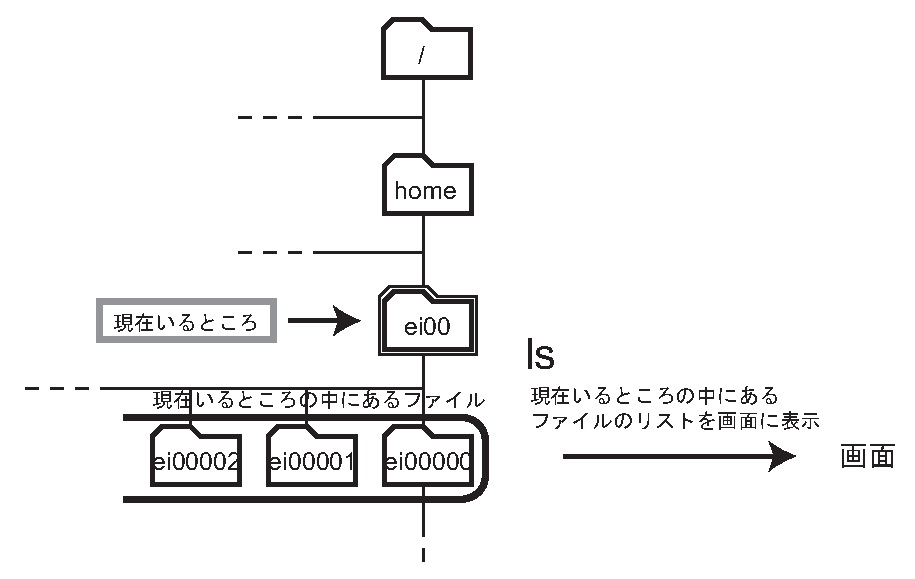
\includegraphics[scale=0.8]{lsdirlist.eps}}
%\caption{「\texttt{cd ..}」で一つ上へ}
\end{figure}

\bigskip

\subsubsection{ファイルの種類を識別: \texttt{ls} の \texttt{-F} オプション}

では、ここで「\texttt{ls -F}」と打ってみよう。

「\texttt{-F}」は「\textbf{f}ile -- ファイル(の種類)」の意味で、
次のようにディレクトリの場合、後ろに「\texttt{/}」を付けて表示してくれるので、
ずいぶん見やすくなる。

\begin{progls}
% \slbfl{ls -F}
ei00001/        ei00010/        ei00019/        ei00028/        ei00037/
ei00002/        ei00011/        ei00020/        ei00029/        ei00038/
ei00003/        ei00012/        ei00021/        ei00030/        ei00039/
ei00004/        ei00013/        ei00022/        ei00031/        ei00040/
ei00005/        ei00014/        ei00023/        ei00032/        ei00041/
ei00006/        ei00015/        ei00024/        ei00033/        ei00042/
ei00007/        ei00016/        ei00025/        ei00034/        ei00043/
ei00008/        ei00017/        ei00026/        ei00035/        ei00044/
ei00009/        ei00018/        ei00027/        ei00036/        ei00045/
%
\end{progls}

「\texttt{ls -F}」の「\texttt{-F}」のように、「\texttt{-なんとか}」のような
形の引数を\textbf{「コマンドのオプション」}という。

コマンドには、それぞれのコマンドによって、いろいろなオプションがある。
そして、オプションを付けると、コマンドの働きを変えることができるように
なっている。
他にどんなオプションがあるかは \texttt{ls} のオンライン・マニュアルに
載っている。

\subsubsection{一気に絶対パスで移動}

次に、 UNIX の最も基本的なコマンドの置いてある「\texttt{/bin}」に
移動してみよう。

\begin{figure}[H]
\centering{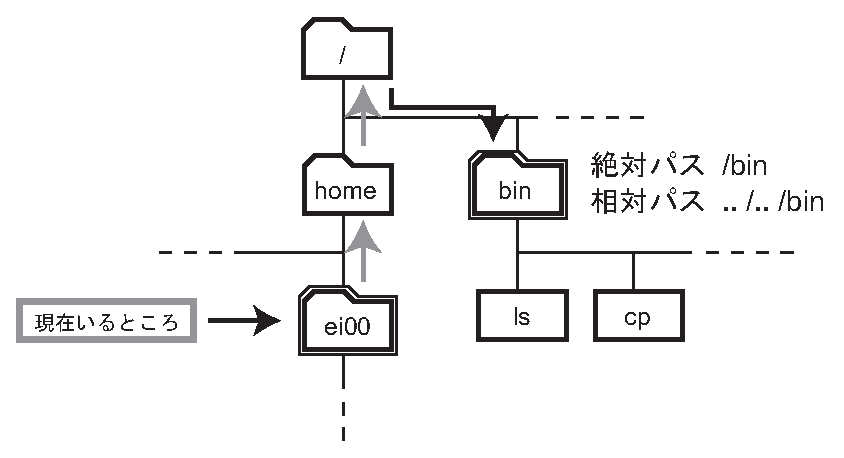
\includegraphics[scale=0.8]{binabrel.eps}}
\end{figure}

これは絶対パスではそのまま「\texttt{/bin}」である。
一方、相対パスで考えると、現在「\texttt{/home/ei00}」にいるので、
「一つ上」の「一つ上」の中にある「\texttt{bin}」ということで、
「\texttt{../../bin}」になる。

つまり、「\texttt{cd /bin}」か「\texttt{cd ../../bin}」だ。
今回は絶対パスの方が簡単なので、こちらを使おう。

\begin{progls}
% \slbfl{cd /bin}
%
\end{progls}

これで、一気に「\texttt{/bin}」まで移動できたはずだ。
 \texttt{pwd} で確認してみよう。

\begin{progls}
% \slbfl{pwd}
/bin
%
\end{progls}

確かに「\texttt{/bin}」にいることがわかる。

では、どんなファイルがあるか \texttt{ls} で見てみよう。

\begin{progls}
% \slbfl{ls}
[               dd              kill            pwd             sleep
cat             df              ln              rcp             stty
chio            domainname      ls              red             sync
chmod           echo            mkdir           rm              test
cp              ed              mv              rmail
csh             expr            pax             rmdir
date            hostname        ps              sh
%
\end{progls}

ここで \texttt{ls -F} すると、次のようになる。
「\texttt{*}」マークは実行できるコマンドの目印である。

\begin{progls}
% \slbfl{ls -F}
[*              dd*             kill*           pwd*            sleep*
cat*            df*             ln*             rcp*            stty*
chio*           domainname*     ls*             red*            sync*
chmod*          echo*           mkdir*          rm*             test*
cp*             ed*             mv*             rmail*
csh*            expr*           pax*            rmdir*
date*           hostname*       ps*             sh*
%
\end{progls}

他のコマンドでも同様なのだが \texttt{cd}には、
ここまで見てきたように、「相対パス」と「絶対パス」の両方が使える。

では、どっち使えばいいのかというと、
「自分のいるとこの近くなら、相対パス」、
「遠くなら絶対パス」が便利なことが多い。

\subsubsection{ホームに戻る}

では、ホーム・ディレクトリに戻ろう。

これはとても簡単で、単に「\texttt{cd}」と打てばいい。
いつ、どこにいても、自分のホーム・ディレクトリには、「\texttt{cd}」と
打つだけで戻れる。

では、やってみよう。

\begin{progls}
% \slbfl{cd}
%
\end{progls}

\begin{figure}[H]
\centering{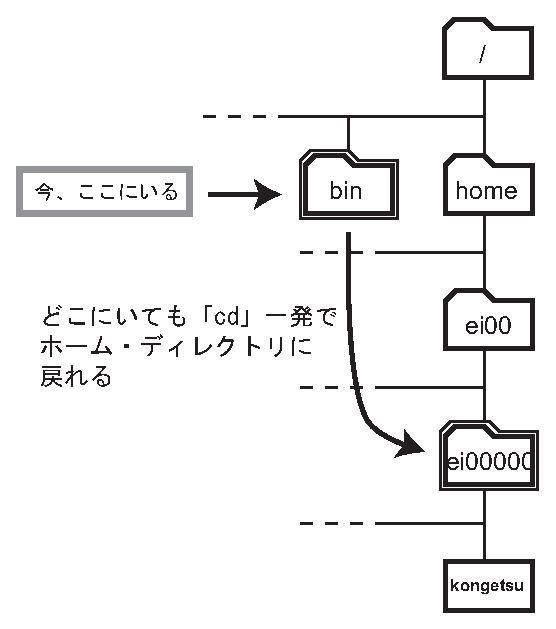
\includegraphics[scale=0.8]{cdhomedir.eps}}
\end{figure}

\newpage

\texttt{pwd} で確認してみよう。

\begin{progls}
% \slbfl{pwd}
/home/ei00/ei00000
%
\end{progls}

確かに、ホーム・ディレクトリに戻れたことがわかる。

\subsubsection{ホームを表す記号: 「\TILDE」}

UNIX システムでは、自分のホーム・ディレクトリを表すのに「\TILDE」を使う。
さきほどの例では、「\texttt{cd}」と単に打ったが、
「\texttt{cd \TILDE}」でも全く同様の効果がある。
では、ためしに使ってみよう。

まず、どこでもいいのだが、
今回は簡単のためルート・ディレクトリ「\texttt{/}」に移動しよう。

\begin{progls}
% \slbfl{cd /}
%
\end{progls}

\texttt{pwd} で確認してみよう。

\begin{progls}
% \slbfl{pwd}
/
%
\end{progls}

確かにルート・ディレクトリ「\texttt{/}」にいることがわかる。

ここから、「\texttt{cd \TILDE}」で自分のホーム・ディレクトリに戻ってみよう。

\begin{progls}
% \slbfl{cd \TILDE}
%
\end{progls}

\texttt{pwd} で確認してみよう。

\begin{progls}
% \slbfl{pwd}
/home/ei00/ei00000
%
\end{progls}

確かにホーム・ディレクトリに戻れた。

「\TILDE」は自分のものだけでなく、他人のホーム・ディレクトリも
「{\TILDE}その人のID」としてやると使うことができる。
たとえば、「\texttt{kokubo}」さんのホーム・ディレクトリは
「\texttt{{\TILDE}kokubo}」、
「\texttt{ei00000}」さんのものは「\texttt{{\TILDE}ei00000}」
となる。

\begin{figure}[H]
\centering{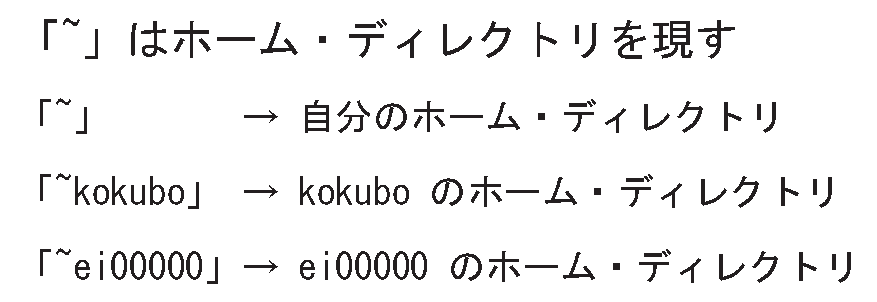
\includegraphics[scale=0.8]{tildehomedir.eps}}
\end{figure}
%\newpage

\subsection{ディレクトリを作る: \texttt{mkdir}}

ディレクトリを作るには \texttt{mkdir} だ。
これは「\textbf{m}ake \textbf{dir}ectory -- メイク・ディレクトリ」
の短縮形である。
使い方は次の通り。

\begin{coml}{10cm}
\texttt{mkdir} 「作りたいディレクトリの名前」
\end{coml}

では、自分のホームの下に「\texttt{prog}」というディレクトリを作ってみよう。

\begin{progls}
% \slbfl{mkdir prog}
%
\end{progls}

\begin{figure}[H]
\centering{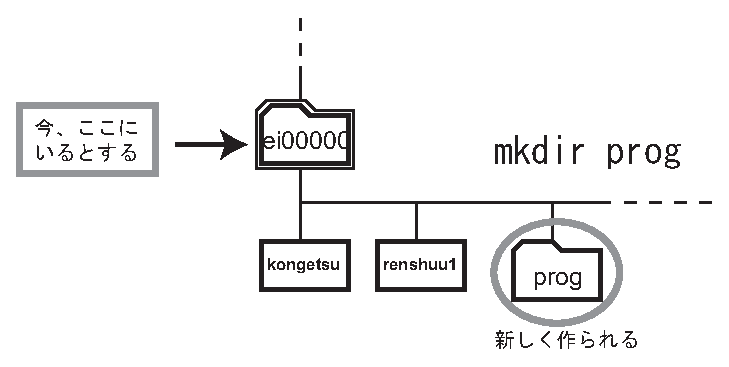
\includegraphics[scale=0.8]{mkdirprog.eps}}
\end{figure}

では、 \texttt{ls} で確認してみよう。

\begin{progls}
% \slbfl{ls}
2000nen         3years          kotoshi         renshuu1.ps     thismonth
2001nen         4gatsu          prog            renshuu2
2002nen         kongetsu        renshuu1        tanjoubi
%
\end{progls}

これでは、「\texttt{prog}」があるのはわかるが、ファイルかディレクトリか
区別がつかない。

区別をはっきりつけるには \texttt{ls -F} と打つ。

\begin{progls}
% \slbfl{ls -F}
2000nen         3years          kotoshi         renshuu1.ps     thismonth
2001nen         4gatsu          prog/           renshuu2
2002nen         kongetsu        renshuu1        tanjoubi
%
\end{progls}

たしかに、「\texttt{prog}」というディレクトリがあるのがわかる。

では、「\texttt{prog}」の中に入ってみよう。
これは、絶対パスなら「\texttt{/home/ei00/ei00000/prog}」で、
相対パスでは単に「\texttt{prog}」なので、相対パスの方が簡単だ。
よって、「\texttt{cd prog}」と打とう。

\begin{progls}
% \slbfl{cd prog}
%
\end{progls}

では、 \texttt{pwd} で確認してみよう。

\begin{progls}
% \slbfl{pwd}
/home/ei00/ei00000/prog
%
\end{progls}

\begin{figure}[H]
\centering{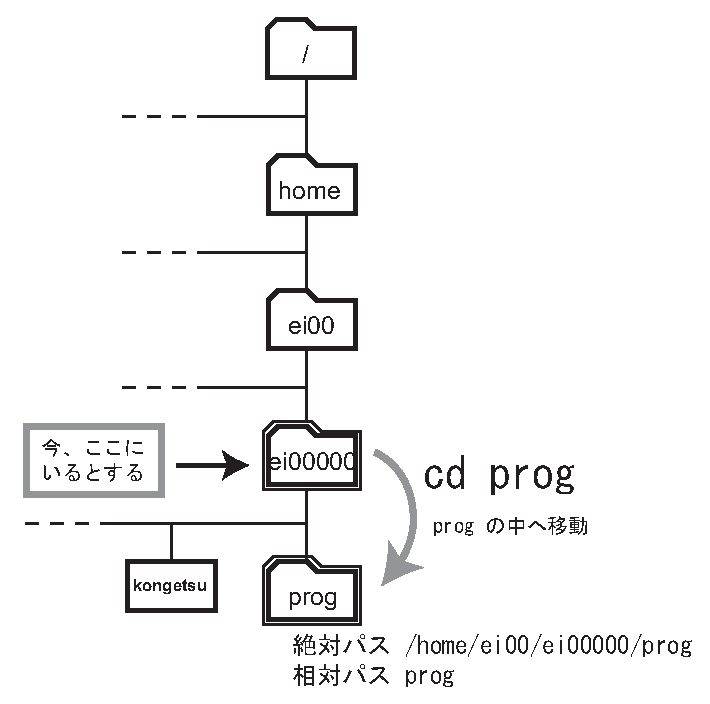
\includegraphics[scale=0.8]{cdprog.eps}}
\end{figure}

\newpage

\subsection{ディレクトリを消す: \texttt{rmdir}}

ディレクトリを消すには、 \texttt{rmdir} だ。
これは「\textbf{r}e\textbf{m}ove \textbf{dir}ectory -- ディレクトリ削除」の
略である。
使い方は次の通りだ。

\begin{coml}{10cm}
\texttt{rmdir} 「消したいディレクトリの名前」
\end{coml}

では、実際にやってみよう。
まず、自分のホーム・ディレクトリにもどろう。
ホームに戻るには単に \texttt{cd} でいい。

\begin{progls}
% \slbfl{cd}
%
\end{progls}

次のように \texttt{pwd} で確認すると、確かにホームにいることがわかる。

\begin{progls}
% \slbfl{pwd}
/home/ei00/ei00000
%
\end{progls}

では、 \texttt{ls -F} でファイルのリストを確認しよう。

\begin{progls}
% \slbfl{ls -F}
2000nen         3years          kotoshi         renshuu1.ps     thismonth
2001nen         4gatsu          prog/           renshuu2
2002nen         kongetsu        renshuu1        tanjoubi
%
\end{progls}

ここにある「\texttt{prog}」というディレクトリを次のように
して消してみる。

\begin{progls}
% \slbfl{rmdir prog}
%
\end{progls}

これで、消えたはずだ。
\texttt{ls -F} で確認してみよう。

\begin{progls}
% \slbfl{ls -F}
2000nen         3years          kotoshi         renshuu2
2001nen         4gatsu          renshuu1        tanjoubi
2002nen         kongetsu        renshuu1.ps     thismonth
%
\end{progls}

確かに消えている。

\bigskip

注・ディレクトリの中に何かファイルが残っていると、 \texttt{rmdir} で
ディレクトリを消すことはできない。

\begin{figure}[H]
\centering{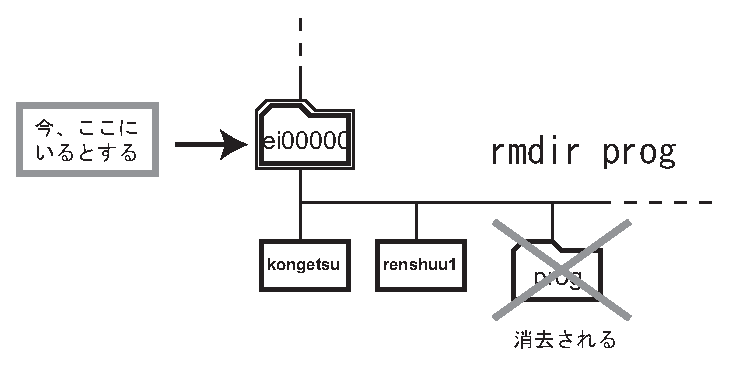
\includegraphics[scale=0.8]{rmdirprog.eps}}
\end{figure}

%\newpage

\subsection{ディレクトリ間でのファイルの移動、コピー}

\texttt{mv} や \texttt{cp} で別のディレクトリにファイルを移動したり、
コピーする方法を紹介しよう。

\bigskip

まず、その前に準備をしよう。
「\texttt{prog}」というディレクトリがあるかどうかを確認する。

\begin{progls}
% \slbfl{ls -F}
2000nen         3years          kotoshi         renshuu2
2001nen         4gatsu          renshuu1        tanjoubi
2002nen         kongetsu        renshuu1.ps     thismonth
%
\end{progls}

もしも、上のように「\texttt{prog}」がないなら、
\texttt{mkdir} で作る。

\begin{progls}
% \slbfl{mkdir prog}
%
\end{progls}

では、 \texttt{ls -F} でファイルのリストを確認しよう。

\begin{progls}
% \slbfl{ls -F}
2000nen         3years          kotoshi         renshuu1.ps     thismonth
2001nen         4gatsu          prog/           renshuu2
2002nen         kongetsu        renshuu1        tanjoubi
%
\end{progls}

確かに「\texttt{prog}」ができていることがわかる。
これで準備は OK である。

%\bigskip
\newpage

「\texttt{prog}」というディレクトリに
「\texttt{renshuu1}」というファイルをコピーしたいとする。

ファイルをディレクトリの中に移動やコピーする場合でも、
 \texttt{mv} や \texttt{cp} の使い方は、普通に移動したりコピーするときと
基本的には同じである。
ファイル名の部分にパスを書いてあげればいい。

つまり、「\texttt{renshuu1}」を「\texttt{prog}」の下に同じ名前で
コピーするには、「\texttt{cp renshuu1 prog/renshuu1}」となる。

また、今回のようにコピー先の名前がコピー元と同じ場合には省略可能で、
「\texttt{cp renshuu1 prog/}」や「\texttt{cp renshuu1 prog}」
としても OK である。

\begin{figure}[H]
\centering{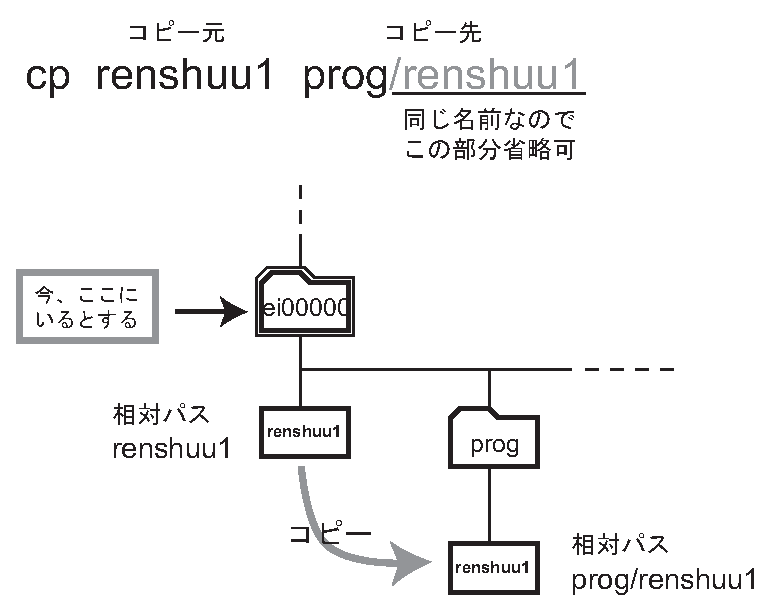
\includegraphics[scale=0.8]{cpunderprog.eps}}
\end{figure}

では、実際にやってみよう。

\begin{progls}
% \slbfl{cp renshuu1 prog}
%
\end{progls}

\bigskip

うまくコピーできたか確かめてみよう。
「\texttt{prog}」の中に移動し、
\texttt{ls -F} で確かめてみると、たしかに「\texttt{renshuu1}」ができている

\begin{progls}
% \slbfl{cd prog}
% \slbfl{ls -F}
renshuu1
%
\end{progls}

\newpage

それでは、「\texttt{prog}」の中の「\texttt{renshuu1}」を、
一つ上のディレクトリ(この場合はホーム・ディレクトリ)に
「\texttt{renshuu3}」という名前で移動してみよう。

現在、「\texttt{prog}」の中にいるので、移動元が「\texttt{renshuu1}」で、
移動先は相対パスで「\texttt{../renshuu3}」となる。
よって、「\texttt{mv renshuu1 ../renshuu3}」である。

\begin{progls}
% \slbfl{mv renshuu1 ../renshuu3}
%
\end{progls}

まず、「\texttt{prog}」の中でファイルのリストを表示してみると、
「\texttt{renshuu1}」がなくなっていることがわかる。

\begin{progls}
% \slbfl{ls}
%
\end{progls}

次に、ホーム・ディレクトリにもどって確認してみると、
確かに「\texttt{renshuu3}」ができていることがわかる。

\begin{progls}
% \slbfl{cd ..}
% \slbfl{ls -F}
2000nen         3years          kotoshi         renshuu1.ps     tanjoubi
2001nen         4gatsu          prog/           renshuu2        thismonth
2002nen         kongetsu        renshuu1        renshuu3
%
\end{progls}

\begin{figure}[H]
\centering{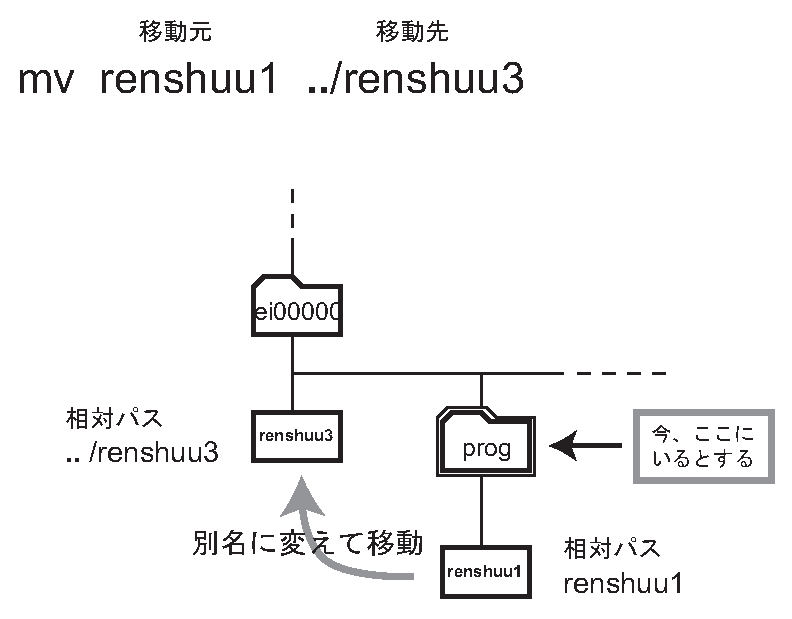
\includegraphics[scale=0.8]{mvoverprog.eps}}
\end{figure}

\newpage

\subsection{移動という言葉}

UNIX コマンドで \texttt{mv} と言えば「ファイルを\textbf{移動}」、
\texttt{cd} と言えば「ディレクトリを\textbf{移動}」で、
どちらも日本語では同じ「\textbf{移動}」である。

この 2 つの違いは、とても簡単で、
「\texttt{mv} は\textbf{ファイルなどを}移動する」、
「\texttt{cd} は\textbf{自分が}移動する」ということである。

\texttt{mv} では、自分は動かないで、動くのはファイルである。
一方、 \texttt{cd} では、自分が移動して、ファイルなどは動かないのだ。

\begin{figure}[H]
\centering{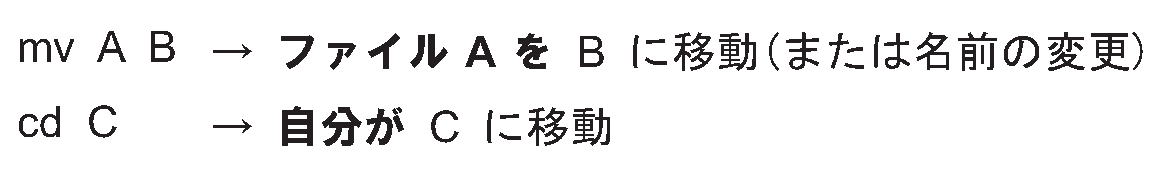
\includegraphics[scale=0.8]{mvcd.eps}}
\end{figure}

\section*{この章で紹介したコマンド}

\begin{center}
\begin{minipage}{13cm}
\begin{itembox}[l]{ディレクトリ操作コマンド}
\begin{description}
\item[\texttt{pwd} :] 自分が現在いる場所を表示

使い方: \texttt{pwd}
\item[\texttt{cd} :] ディレクトリを移動する

使い方: \texttt{cd 「パス名」}
\item[\texttt{mkdir} :] ディレクトリの作成

使い方: \texttt{mkdir} 「ディレクトリ名」
\item[\texttt{rmdir} :] ディレクトリの削除

使い方: \texttt{rmdir} 「ディレクトリ名」
\end{description}
\end{itembox}
\end{minipage}
\end{center}

\subsubsection{問題の解答}
\begin{figure}[H]
\centering{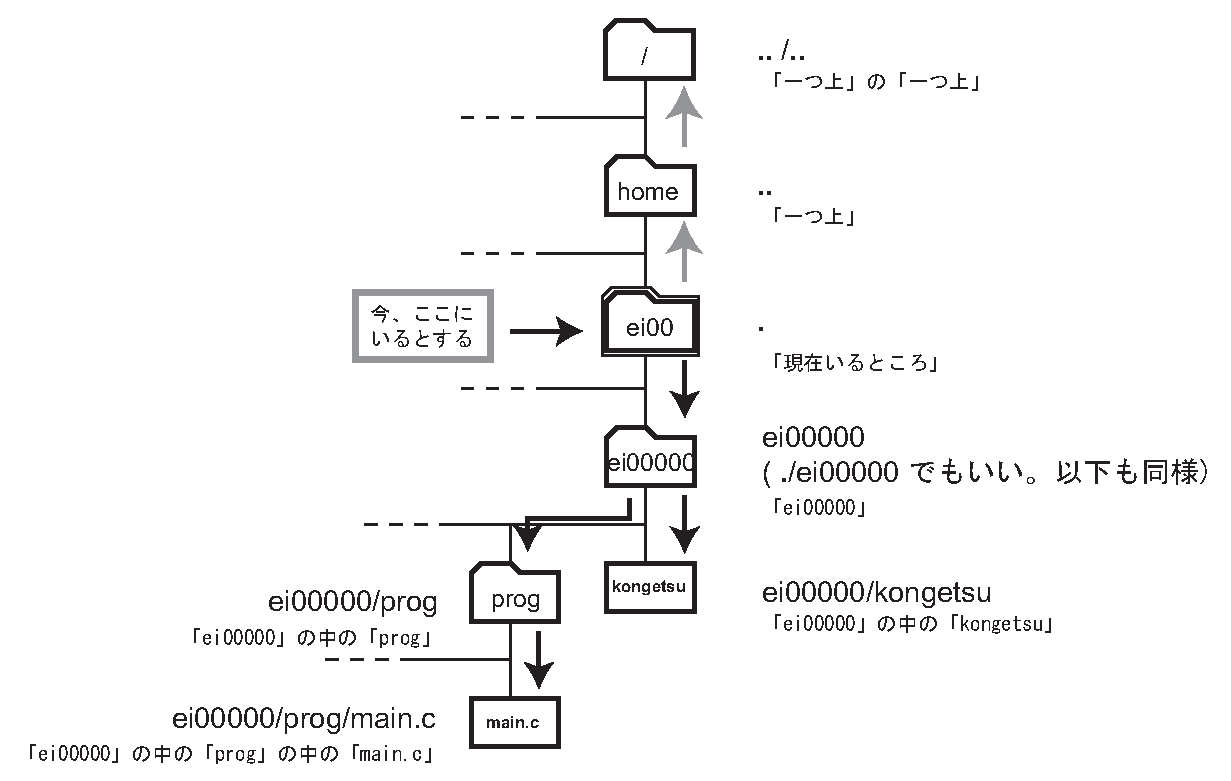
\includegraphics[scale=0.8]{relativepath05.eps}}
\end{figure}

\newpage
{~}
